\subsection{Binary Exactness and Frontend Loss}

On the frozen CelebA roots, all 1,310,720 tested re-keyed bits and 1,310,720 protected probe/gallery scores agree with their reference across 20 epochs. This is exactness relative to the binary frontend.

On the exactly recovered fixed CelebA gallery/probe images, float Rank-1/Rank-5 are 0.8691/0.9473, versus binary 0.8516/0.9375. Twenty paired splits on the historical portability cohort give mean float/binary Rank-1 0.8762/0.8515. The paired binary-minus-float difference is -2.471 percentage points (identity-bootstrap 95\% interval [-3.281, -1.729]). The supplement states the historical reproduction outcome.

\begin{table}[t]
\caption{Paired LFW closed-set utility over 20 splits. The same 128 identities supply probes at every gallery size.}
\label{tab:utility}\centering\small
\setlength{\tabcolsep}{3pt}
\begin{tabular}{rrrrr}
\toprule
Gallery & Float R1 & Binary R1 & Float R5 & Binary R5 \\
\midrule
128 & 0.9891 & 0.9849 & 0.9979 & 0.9965 \\
256 & 0.9851 & 0.9806 & 0.9970 & 0.9960 \\
512 & 0.9825 & 0.9734 & 0.9954 & 0.9919 \\
1024 & 0.9731 & 0.9641 & 0.9934 & 0.9891 \\
2048 & 0.9620 & 0.9496 & 0.9887 & 0.9847 \\
4096 & 0.9531 & 0.9367 & 0.9820 & 0.9761 \\
\bottomrule
\end{tabular}
\end{table}

\begin{figure*}[t]\centering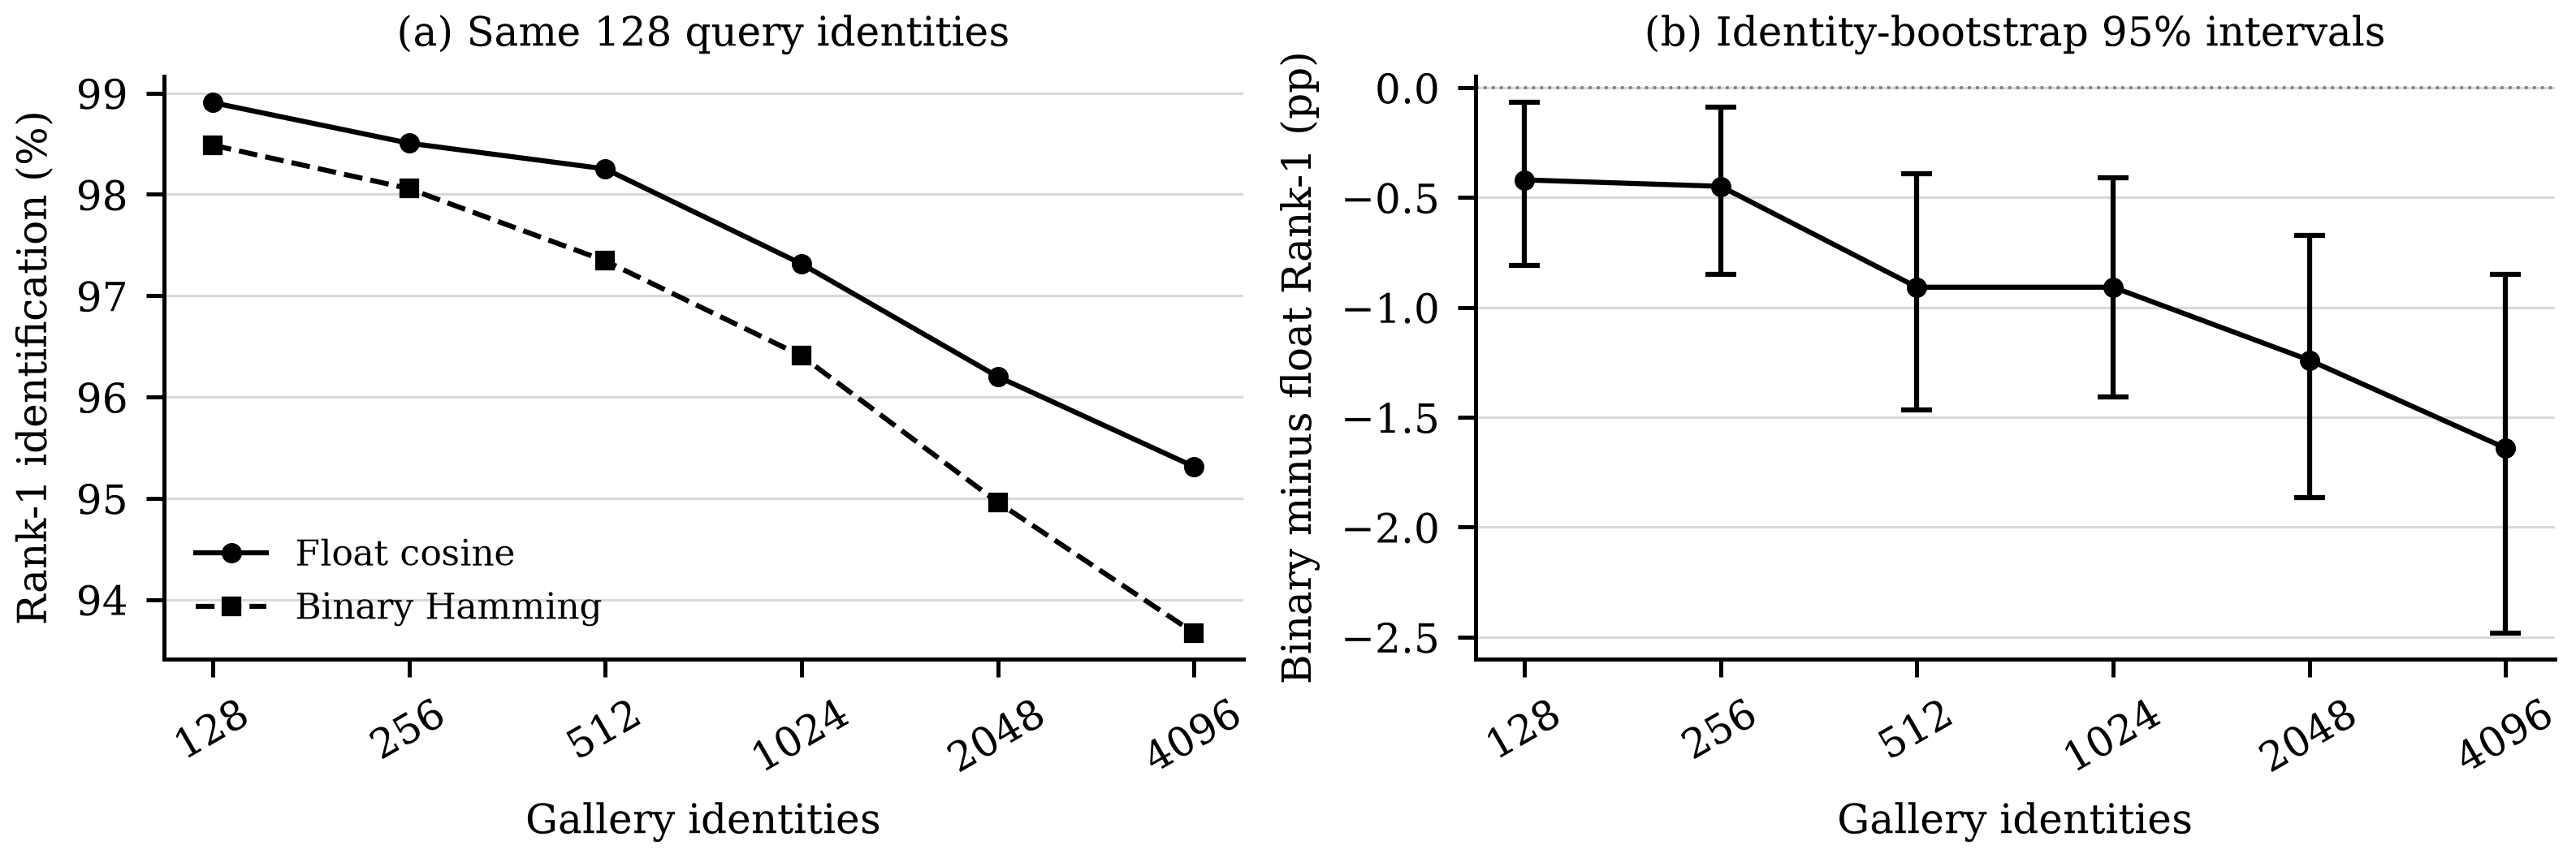
\includegraphics[width=\textwidth]{figures/lfw_paired_scale.png}\caption{Paired utility on nested LFW galleries, using the same 128 query identities and 20 gallery/probe assignments. Additional gallery identities are distractors. Intervals resample query identities after averaging repeated contexts; these are not 4096 independent query subjects.}\label{fig:paired_scale}\end{figure*}

At 128 identities, binarization costs 0.420 percentage points in Rank-1. At 4096, the loss is 1.641 points (binary-minus-float 95\% interval [-2.480, -0.850]). Masking adds no further score error, but it does not recover this frontend loss.

\subsection{Unenrolled Probes and Candidate Behavior}

\begin{table}[t]
\caption{Fresh-unknown LFW test: 512 calibration and 512 disjoint unknown identities. FPIR and DIR are percentages; rules are defined before feature extraction.}
\label{tab:open}\centering\small
\setlength{\tabcolsep}{3pt}
\begin{tabular}{rlrrr}
\toprule
Gallery & Root & Rule & FPIR & DIR \\
\midrule
128 & Float & Emp. & 1.602 & 89.26 \\
128 & Float & Cons. & 0.371 & 79.92 \\
128 & Binary & Emp. & 1.885 & 87.76 \\
128 & Binary & Cons. & 0.537 & 80.01 \\
4096 & Float & Emp. & 1.953 & 71.70 \\
4096 & Float & Cons. & 0.420 & 53.83 \\
4096 & Binary & Emp. & 1.172 & 59.12 \\
4096 & Binary & Cons. & 0.391 & 46.33 \\
\bottomrule
\end{tabular}
\end{table}

The nominal 1\% empirical calibration rule does not guarantee 1\% test FPIR. Conservative thresholds reduce false positives at a substantial DIR cost (Table~\ref{tab:open}). Identity-level intervals and all intermediate gallery sizes are retained in the supplement. The earlier 32-identity frequent-image pilot has test FPIR 5.34\% (float) and 7.19\% (binary) at its nominal 1\% target. This distinct hard population is not replaced or pooled with the confirmation cohort.

\begin{table}[t]
\caption{Unbounded candidate union on one frozen LFW split. Capacity-failing rows are diagnostics, not admitted secure indices.}
\label{tab:index}\centering\small
\setlength{\tabcolsep}{3pt}
\begin{tabular}{rrrrrr}
\toprule
Gallery & $w$ & Recall & Agreement & Fraction & Fallback \\
\midrule
128 & 4 & 1.0000 & 1.0000 & 0.9980 & 0.0566 \\
128 & 8 & 0.9941 & 0.9980 & 0.3049 & 0.9570 \\
4096 & 4 & 1.0000 & 1.0000 & 0.9980 & 0.1758 \\
4096 & 8 & 0.9941 & 0.9980 & 0.2893 & 0.9570 \\
\bottomrule
\end{tabular}
\end{table}

Four-bit buckets retrieve almost the complete gallery. At 4096 identities, eight-bit buckets retrieve about 29\%, but the exactness certificate invokes fallback on 95.70\% of probes. Their public capacity is 72 versus a required 138, with 59 overflowing buckets; enrollment must reject or reconfigure. The certified policy agrees with exhaustive decisions for every evaluated probe. The secure reference hides its choice by computing the full schedule, so candidate pruning is not a measured speedup.

\subsection{Relation Integrity and Leakage Diagnostics}

All eight injected faults are rejected, the previous logical state is retained, and the post-rejection query agrees with the independent oracle. Primitive tests also agree at full field width. In the retained SHAKE simulation, direct linkage AUC is 0.4948, direct assignment 0.0066 and relational assignment 0.0082, against chance 1/128 for assignment; the global-mask relational control is 1.0000. These are attack-specific observations, not an exposed-key or general irreversibility proof.

\subsection{Complete Secure Cost}

\begin{table}[t]
\caption{Input-inclusive five-party masked-system reference: mean and sample SD of three VM timings, global traffic (MB) and largest-child peak RSS (MiB). Five colocated processes; no WAN claim.}
\label{tab:secure}\centering\small
\setlength{\tabcolsep}{3pt}
\begin{tabular}{rlrrr}
\toprule
$N$ & Operation & Seconds & MB & RSS \\
\midrule
8 & Re-key & 9.82$\pm$1.30 & 471.8 & 38.7 \\
8 & Query & 2.28$\pm$0.05 & 10.9 & 27.6 \\
16 & Re-key & 10.05$\pm$0.35 & 722.6 & 48.3 \\
16 & Query & 1.71$\pm$0.25 & 18.3 & 32.9 \\
32 & Re-key & 12.41$\pm$1.51 & 997.3 & 60.0 \\
32 & Query & 2.08$\pm$0.40 & 33.2 & 38.0 \\
64 & Re-key & 16.77$\pm$0.19 & 1564.0 & 93.5 \\
64 & Query & 2.30$\pm$0.07 & 63.4 & 53.0 \\
128 & Re-key & 28.54$\pm$2.37 & 2717.4 & 132.8 \\
128 & Query & 4.09$\pm$0.35 & 122.5 & 63.1 \\
256 & Re-key & 44.02$\pm$0.31 & 5051.5 & 209.6 \\
256 & Query & 8.35$\pm$0.42 & 245.0 & 89.5 \\
\bottomrule
\end{tabular}
\end{table}

\begin{table}[t]
\caption{Complete lifecycle from each party's own persisted share file. Mean and sample SD of three measured VM timings; global MB. No plaintext database/index or old keys are resupplied to a computing party.}
\label{tab:persisted}\centering\small
\setlength{\tabcolsep}{3pt}
\begin{tabular}{rllrr}
\toprule
$N$ & State & Operation & Seconds & MB \\
\midrule
8 & Masked & Re-key & 10.73$\pm$2.15 & 470.7 \\
8 & Shared root & Re-key & 7.84$\pm$0.84 & 453.6 \\
8 & Masked & Query & 2.24$\pm$0.28 & 10.8 \\
8 & Shared root & Query & 0.40$\pm$0.07 & 0.9 \\
128 & Masked & Re-key & 40.76$\pm$6.51 & 2710.0 \\
128 & Shared root & Re-key & 30.36$\pm$4.51 & 2485.3 \\
128 & Masked & Query & 6.63$\pm$1.55 & 120.4 \\
128 & Shared root & Query & 1.22$\pm$0.21 & 14.6 \\
\bottomrule
\end{tabular}
\end{table}

The persisted-state implementation loads the complete public-size bundle before computing. Its helper functions and transition/query tail are source-identical to the input-inclusive reference; only the state entry point differs. Initialization uses an external trusted fixture that sends each party one degree-two Shamir evaluation per field. Repeated re-keying and reload queries agree with the oracle; exact/reject controls and rollback followed by reload also pass. The fixture is outside the computing-party corruption model.

At $N=128$, logical masked state is 3.506 MiB per party before serialization. Phase timers separate locator/index evolution, old/new masks, verification, selection, shuffle/refresh and fresh query masks; the supplement gives all components and wall times.

\begin{table}[t]
\caption{Input-inclusive same-configuration baselines and private indexed-query reference. Three measured runs after warmup; mean and sample SD. Full phase details accompany the logs.}
\label{tab:baselines}\centering\small
\setlength{\tabcolsep}{3pt}
\begin{tabular}{rllrr}
\toprule
$N$ & Design & Operation & Seconds & MB \\
\midrule
8 & Raw roots & Re-key & 5.74$\pm$0.27 & 454.8 \\
8 & Raw roots & Query & 0.50$\pm$0.16 & 1.0 \\
8 & Private index & Query & 43.28$\pm$0.86 & 4965.0 \\
32 & Raw roots & Re-key & 11.03$\pm$1.15 & 939.1 \\
32 & Raw roots & Query & 0.48$\pm$0.03 & 4.2 \\
128 & Raw roots & Re-key & 22.49$\pm$0.54 & 2492.7 \\
128 & Raw roots & Query & 0.91$\pm$0.05 & 16.7 \\
8 & Compact sort & Re-key & 93.88$\pm$22.51 & 7274.6 \\
16 & Compact sort & Re-key & 127.35$\pm$4.56 & 15788.2 \\
\bottomrule
\end{tabular}
\end{table}

An input-inclusive cost model fitted only at $N=8,16,32$ is checked on held-out measured sizes. Maximum relative error is 1.5\% for global communication and 86.9\% for local VM time. Exact residuals are reported even when the model is inaccurate; we make no extrapolated runtime claim at 4096. This model excludes persisted-file loading. The biometric 4096-gallery study is separate from measured MPC scale.
